
\documentclass[12pt]{article}
 
\usepackage[margin=1in]{geometry} 
\usepackage{amsmath,amsthm,amssymb}
\usepackage{pifont}
\usepackage{graphics}
\usepackage{graphicx}
\usepackage{array}
 
\newcommand{\N}{\mathbb{N}}
\newcommand{\Z}{\mathbb{Z}}
 
\newenvironment{theorem}[2][Theorem]{\begin{trivlist}
\item[\hskip \labelsep {\bfseries #1}\hskip \labelsep {\bfseries #2.}]}{\end{trivlist}}
\newenvironment{lemma}[2][Lemma]{\begin{trivlist}
\item[\hskip \labelsep {\bfseries #1}\hskip \labelsep {\bfseries #2.}]}{\end{trivlist}}
\newenvironment{exercise}[2][Exercise]{\begin{trivlist}
\item[\hskip \labelsep {\bfseries #1}\hskip \labelsep {\bfseries #2.}]}{\end{trivlist}}
\newenvironment{problem}[2][Problem]{\begin{trivlist}
\item[\hskip \labelsep {\bfseries #1}\hskip \labelsep {\bfseries #2.}]}{\end{trivlist}}
\newenvironment{question}[2][Question]{\begin{trivlist}
\item[\hskip \labelsep {\bfseries #1}\hskip \labelsep {\bfseries #2.}]}{\end{trivlist}}
\newenvironment{corollary}[2][Corollary]{\begin{trivlist}
\item[\hskip \labelsep {\bfseries #1}\hskip \labelsep {\bfseries #2.}]}{\end{trivlist}}

\newenvironment{solution}{\begin{proof}[Solution]}{\end{proof}}
 
\begin{document}
 
% --------------------------------------------------------------
%                         Start here
% --------------------------------------------------------------
 
\title{Homework 4}
\author{Jia Guo, Georgios Kontoudis\\ 
ME5774 Nonlinear Systems Theory\\
Professor Cornel Sultan} 
\date{Fall 2017}
 
\maketitle
\begin{problem}{1} %theorem, exercise, problem, or question 
%Determine if the equilibrium $x_1=x_2=0$ is unstable, stable, asymptotically stable, exponentially stable for
%\begin{align*}
%&\dot{x_1}=x_2-x_1^3+x_1^5 \\
%&\dot{x_2}=-x_1,
%\end{align*}
%where $\textbf{x}=[x_1 \quad x_2]^\top \in \mathbb{R}^2$. State the strongest claim you can make and provide support for the conclusion. You can consider only local properties.
\end{problem}
\begin{solution}
Consider the system
\begin{align*}
&\dot{x_1}= \tanh x_1 (ax_1+x_2) \\
&\dot{x_2}=bx_1x_2+ \frac{1}{1+x_2^2}u,
\end{align*}
where $a=2$, $b=3$ are the determined values of the model. The proper form for integrator backstepping is
\begin{align}\label{eta_zeta}
&\dot{x_1}= 2x_1 \tanh x_1 +x_2 \tanh x_1 \\
&\dot{x_2}=3x_1x_2+ \frac{1}{1+x_2^2}u.
\end{align}
The system has an equilibrium at the origin $\textbf{x}_e=[0 \quad 0]^{\top}$. Let us define $x_2= \phi (x_1)=-2x_1-x_1^2$. From Equation~\ref{eta_zeta} we get the closed-loop system
\begin{align*}
&\dot{x}_1= -x_1^2 \tanh x_1 .
\end{align*}
Let us consider the Lyapunov function $V=\frac{1}{2}x_1^2>0$, where the rate of change yields
\begin{equation*}
\begin{aligned}
& \dot{V}
& = 
&&& x_1\dot{x}_1\\
&&=
&&& x_1(-x_1^2 \tanh x_1)\\
&&=
&&&-x_1^3 \tanh x_1.
\end{aligned}
\end{equation*}
If $x_1>0$ then $\tanh x_1>0$, so $-x_1^3 \tanh x_1<0$. On the other hand, if $x_1<0$ then $\tanh x_1<0$, so $-x_1^3 \tanh x_1<0$. Next, if $x_1=0$ then  $-x_1^3 \tanh x_1=0$. So $\dot{V} \leq -W(x_1)$, where $W(x_1)=x_1^3 \tanh x_1$ is a positive definite function for all $\textbf{x} \in \mathbb{R}^2- \{ \textbf{0} \}$. Since the Lyapunov function is radially unbounded, because $V \rightarrow \infty \mbox{ as } \| \textbf{x}\| \rightarrow \infty$, we have a globally asymptotically stable equilibrium at the origin $\textbf{x}_e$.

Let us consider the augmented Lyapunov function
\begin{align*}
V_a= V +\frac{1}{2}(x_2- (-2x_1-x_1^2))^2,
\end{align*}
where by choosing the control $u$ as
\begin{align}\label{control_u}
u= (1+x_2^2)(-3x_1x_2+ \frac{\partial \phi}{\partial x_1}(2x_1 \tanh x_1 +x_2 \tanh x_1)-(\frac{\partial V}{\partial x_1}\tanh x_1)-K(x_2- (-2x_1-x_1^2))),
\end{align}
with $K>0$ results
\begin{equation*}
\begin{aligned}
& \dot{V}_a
& \leq 
&&& -W(x_1)-K(x_2- \phi(x_1))^2\\
&& \leq
&&& -x_1^3 \tanh x_1 -K(x_2- (-2x_1-x_1^2))^2.
\end{aligned}
\end{equation*}
Since the augmented Lyapunov function $V_a<0$ for all $\textbf{x} \in \mathbb{R}^2- \{ \textbf{0} \}$, we get asymptotic stability of the origin $\textbf{x}_e$ under this feedaback control $u$.

By using Equation~\ref{control_u} we get the closed-loop system in the physical space
\begin{align}\label{eta_zeta}
&\dot{x_1}= 2x_1 \tanh x_1 +x_2 \tanh x_1 \\
&\dot{x_2}=(-2-2x_1)(2x_1 \tanh x_1+x_2 \tanh x_1)-(x_1 \tanh x_1)-K(x_2+2x_1+x_1^2).
\end{align}
In Figure~\ref{fig:x_1-t} the states $x_1$, $x_2$ over time are depicted. Moreover, in Figure~\ref{fig:x_1-x_2} the state $x_1$ over $x_2$ for various gains $K$ is presented.
\begin{figure}[!h]
	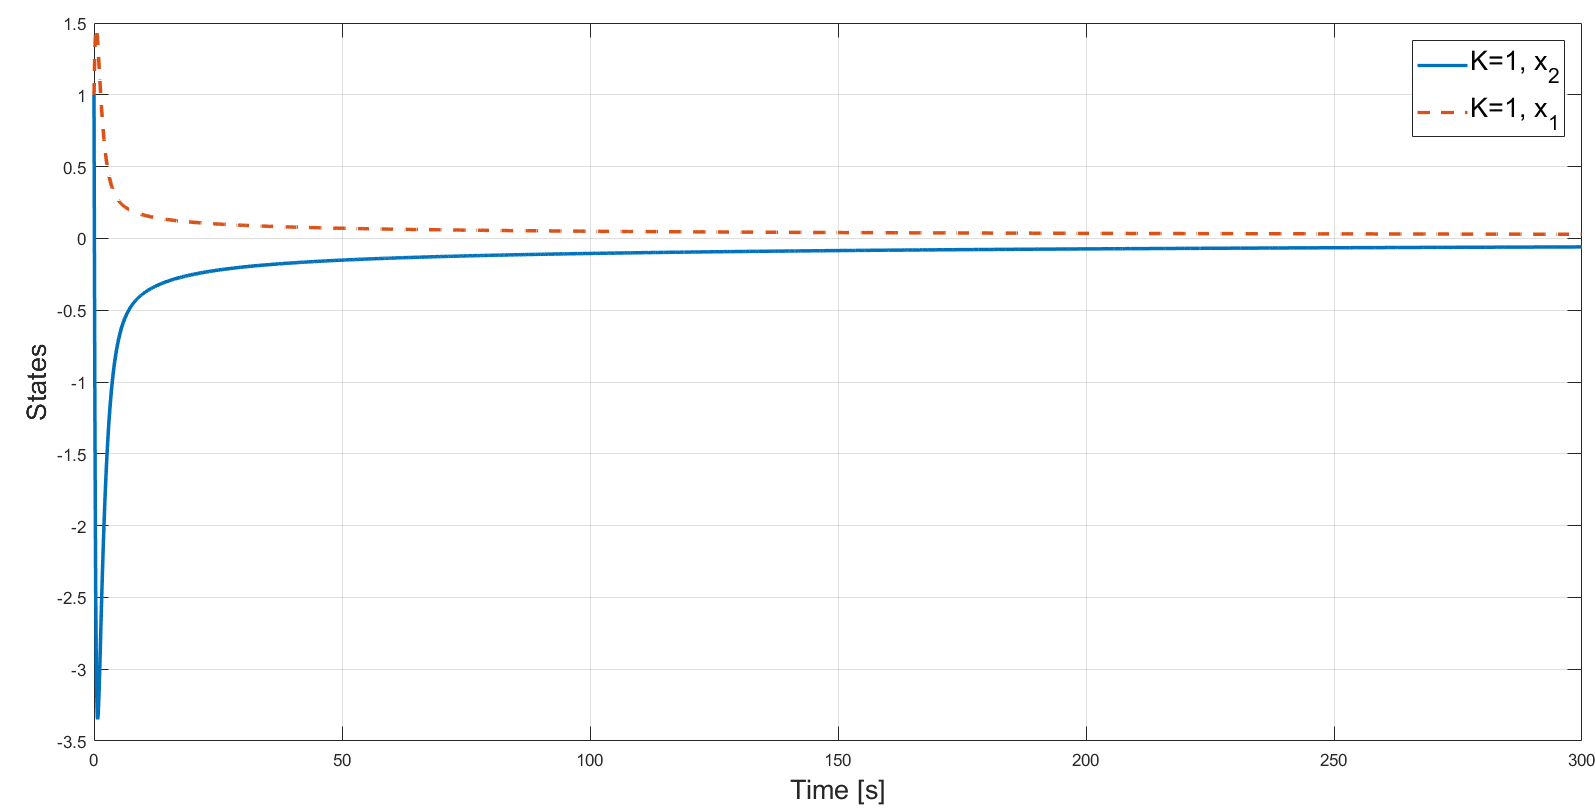
\includegraphics[scale=0.35]{figures/x1_t_p4a.png}
	\centering
	\caption{States $x_1$, $x_2$ over time using backstepping integral for gain $K=1$.}
	\label{fig:x_1-t}
\end{figure}
%\begin{figure}[!h]
%	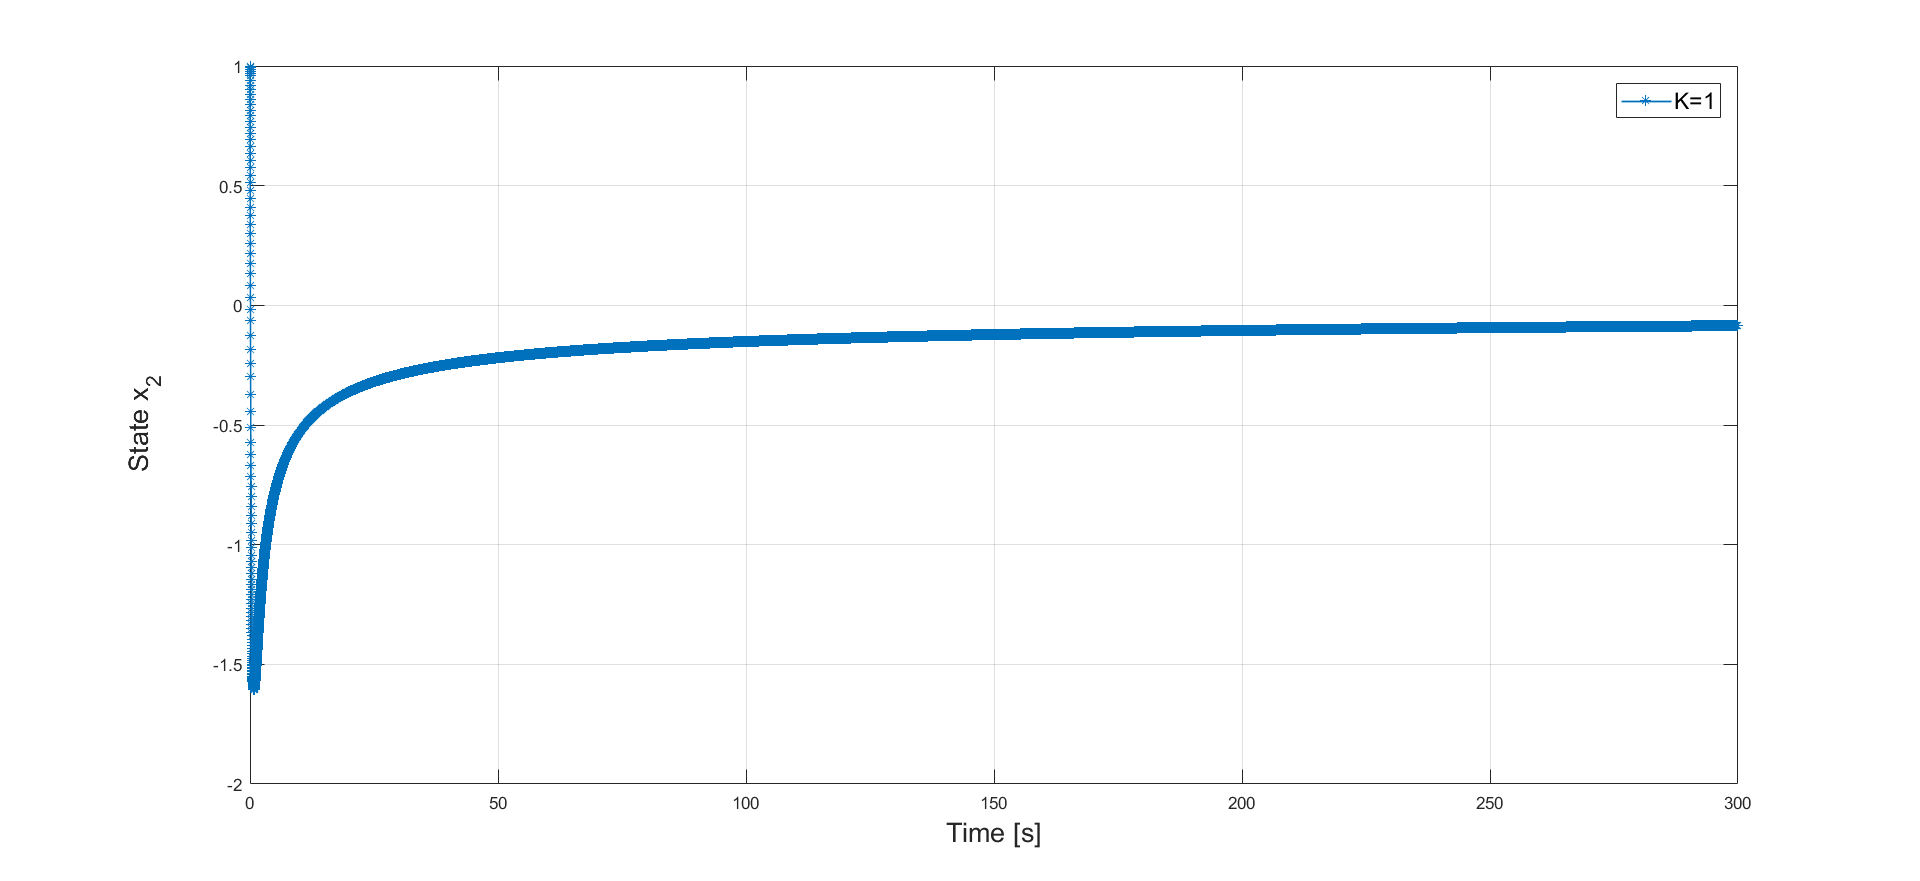
\includegraphics[scale=0.3]{figures/x2_t_p4a.png}
%	\centering
%	\caption{State $x_2$ over time of the closed-loop system using backstepping integral for gain $K=1$.}
%	\label{fig:x_2-t}
%\end{figure}
\begin{figure}[!h]
	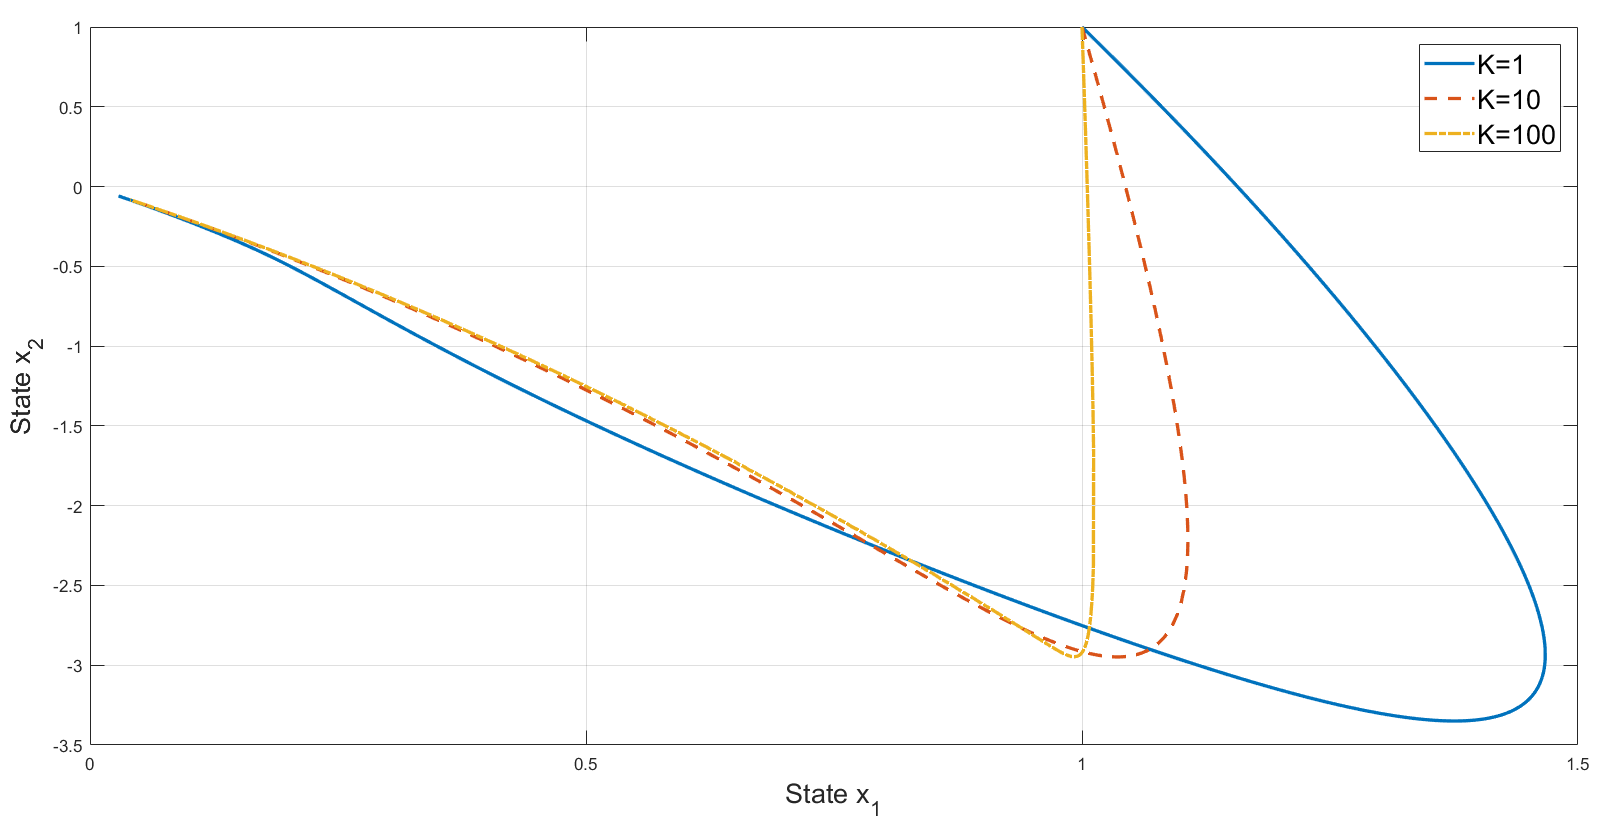
\includegraphics[scale=0.35]{figures/x1_x2_p4a.png}
	\centering
	\caption{State $x_1$ over $x_2$ using backstepping integral for various gain $K$ values.}
	\label{fig:x_1-x_2}
\end{figure}
\end{solution}

%%-----------------------------------------------------------

\begin{problem}{2} %theorem, exercise, problem, or question

\end{problem}

\begin{solution}
Consider the system
\begin{align*}
&\dot{x_1}= \tanh x_1 (ax_1+x_2) \\
&\dot{x_2}=bx_1x_2+ \frac{1}{1+x_2^2}u,
\end{align*}
but in this case the parameters a, b are uncertain. Since we are aware of the bounds $a\in [1,3]$, $b\in [2,4]$ we can extract the nominal parameters $\hat{a}=2$, $\hat{b}=3$. Let us set
\begin{align*}
&a= \hat{a}+a-\hat{a} \\
&b= \hat{b}+b-\hat{b}.
\end{align*}
Then we can formulate the system's equation to the sliding mode control form
\begin{align*}
&\dot{x_1}= \tanh x_1 (( \hat{a}+a-\hat{a} )x_1+x_2)= (\hat{a}x_1+x_2) \tanh x_1 + (a-\hat{a})x_1 \tanh x_1\\
&\dot{x_2}= ( \hat{b}+b-\hat{b} )x_1x_2+ \frac{1}{1+x_2^2}u=\hat{b}x_1x_2+\frac{1}{1+x_2^2}(u+x_1x_2(1+x_2^2)(b-\hat{b})),
\end{align*}
where
\begin{align*}
&f(x_1,x_2)= (\hat{a}x_1+x_2)\tanh x_1, \qquad
\delta_{x_1}=(a-\hat{a})x_1\tanh x_1 
\end{align*}
\begin{align*}
&f_a(x_1,x_2)=\hat{b}x_1x_2, \qquad
G_a(x_2)=\frac{1}{1+x_2^2}, \qquad
\delta(x_2)=x_1x_2(1+x_2^2)(b-\hat{b}).
\end{align*}

Let us choose $x_2=\phi(x_1)=-\hat{a}x_1-\alpha |x_1|=-2x_1-\alpha |x_1|$, where $\alpha>1$. Next, considering the Lyapunov function $V=\frac{1}{2}x_1^2>0$ we compute the rate of change
\begin{equation*}
\begin{aligned}
& \dot{V}
& = 
&&& x_1\dot{x}_1\\
&&=
&&& x_1(2x_1-2x_1- \alpha |x_1|)  \tanh x_1 \\
&&=
&&& - x_1 \alpha |x_1|  \tanh x_1 .
\end{aligned}
\end{equation*}
In problem 1 we have proved that $x_1 \tanh x_1 \geq 0$. Since $\alpha>1$ we get  $- x_1 \alpha |x_1|  \tanh x_1| \leq 0$. Therefore, $\dot{V}>0$ for all $\textbf{x} \in \mathbb{R}^2 - \{ \textbf{0} \}$ which yields asymptotic stability at the origin. We choose $\alpha=3 $.

The control law will have the form
\begin{align}\label{control}
&u= u_{eq}+(1+x_2^2)v,
\end{align} 
where 
\begin{equation}\label{controlEq}
\begin{aligned}
&u_{eq}
&= 
&&& G_a^{-1}(x_1,x_2)(-f_a(x_1,x_2)+\frac{\partial \phi}{\partial x_1}f(x_1,x_2)) \\
&&= 
&&& (1+x_2^2)(-(\hat{b}x_1x_2)+(-\hat{a}-\alpha sign(x_1))(\hat{a}x_1+x_2 \tanh x_1))
\end{aligned}
\end{equation}

Next we define $z=x_2- \phi (x_1)$ and we get the rate of change $\dot{z}=v + \Delta$, where
\begin{align}
&\Delta = x_1x_2(b-\hat{b})+(\hat{a}+\alpha sign(x_1))(a-\hat{a})x_1 \tanh x_1.
\end{align}
For finding a feedback control law that drives $z$ in zero in finite time we work on the maximum value of $\Delta$ as follows
\begin{equation*}
\begin{aligned}
& || \Delta||_{\infty}
& \leq 
&&& ||x_1x_2(b-\hat{b})||_{\infty}+||(\hat{a}+\alpha sign(x_1))(a-\hat{a})x_1 \tanh x_1||_{\infty}\\
&&\leq
&&& |x_1 | |x_2| |1|+ (|2+\alpha|) |1||x_1|\\
&&\leq
&&& |x_1 | |x_2|+ (|2+\alpha|)|x_1|= \rho
\end{aligned}
\end{equation*}
Note that we reduce $|| sign(x_1)||_{\infty}=1$ and  $|| \tanh x_1||_{\infty}=1$.

Next we define $\beta = \rho +c$, where $c>0$ and we let 
\begin{align}\label{controlv}
&v= - \beta sign(x_2- \phi(x_1)).
\end{align}

From the Equations~\ref{control},\ref{controlEq},\ref{controlv} we get the feedback control law of the full system
\begin{align*}
&u 
&= 
&&&(1+x_2^2)[(-\hat{b}x_1x_2)-(\hat{a}+\alpha sign(x_1))(\hat{a}x_1+x_2 \tanh x_1)]+\\
&&
&&& (1+x_2^2)(- (|x_1 | |x_2|+ |2+\alpha||x_1| +c) sign(x_2+\hat{a}x_1+\alpha |x_1|)).
\end{align*}
Next, we replace the signum function with a saturation function to avoid chattering. The saturation function sat$(\frac{y}{\epsilon })$ approaches the signum function when $\epsilon \rightarrow 0$. In Figure~\ref{fig:x_1-x_2-t} the states $x_1$, $x_2$ over time are depicted. Moreover, in Figure~\ref{fig:x_1-x_2-smc} the states $x_1$, $x_2$ are presented by employing the signum function and the saturation with various $\epsilon $ values.
\begin{figure}[!h]
	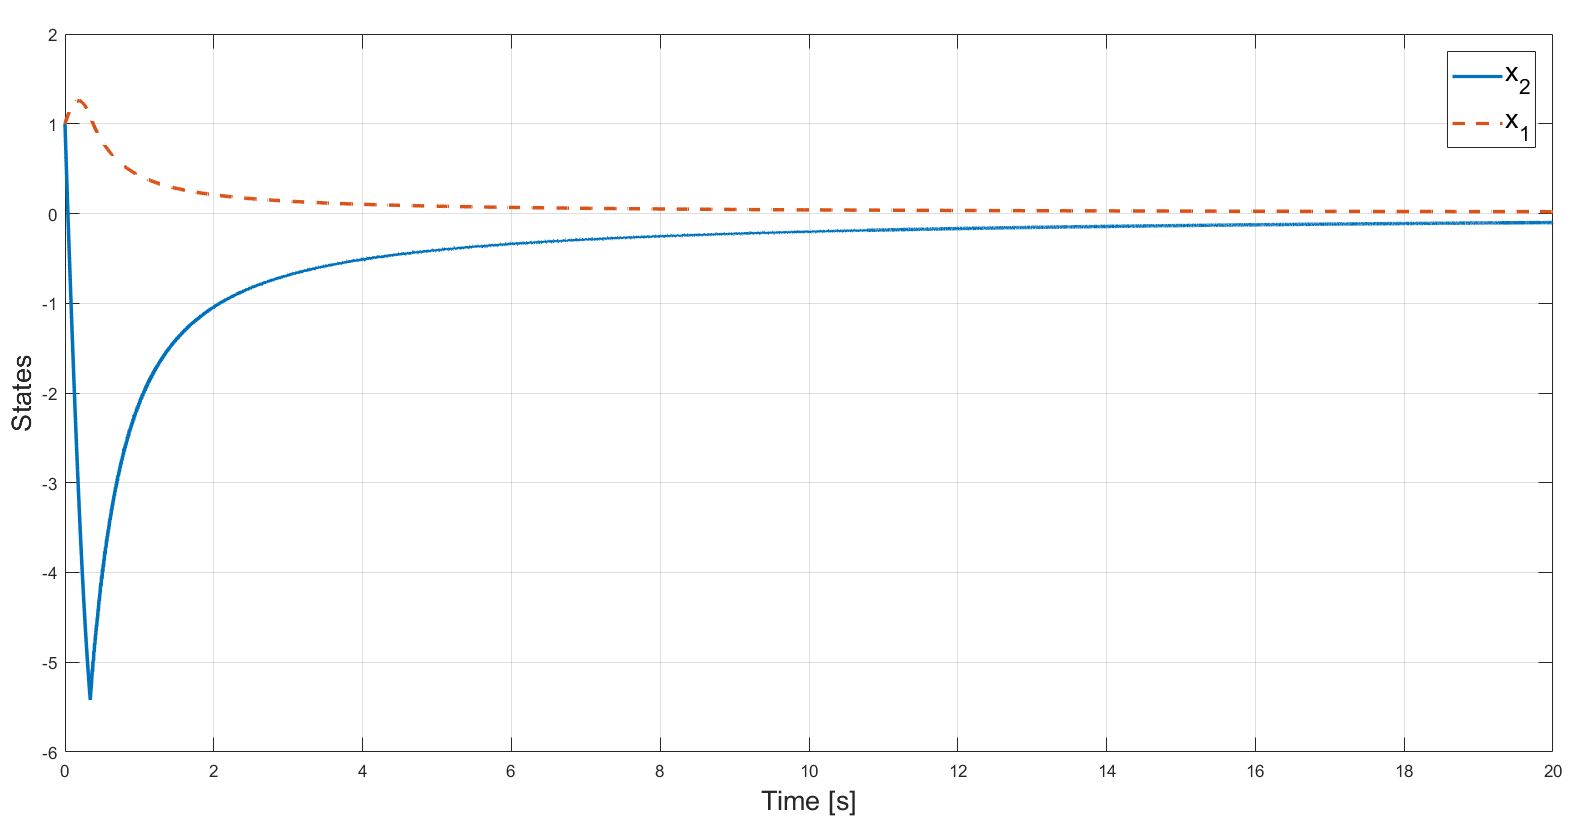
\includegraphics[scale=0.35]{figures/x1_x2_t_p4b.png}
	\centering
	\caption{States $x_1$, $x_2$ over time of the closed-loop system using sliding mode control for gain $K=0$.}
	\label{fig:x_1-x_2-t}
\end{figure}
\begin{figure}[!t]
	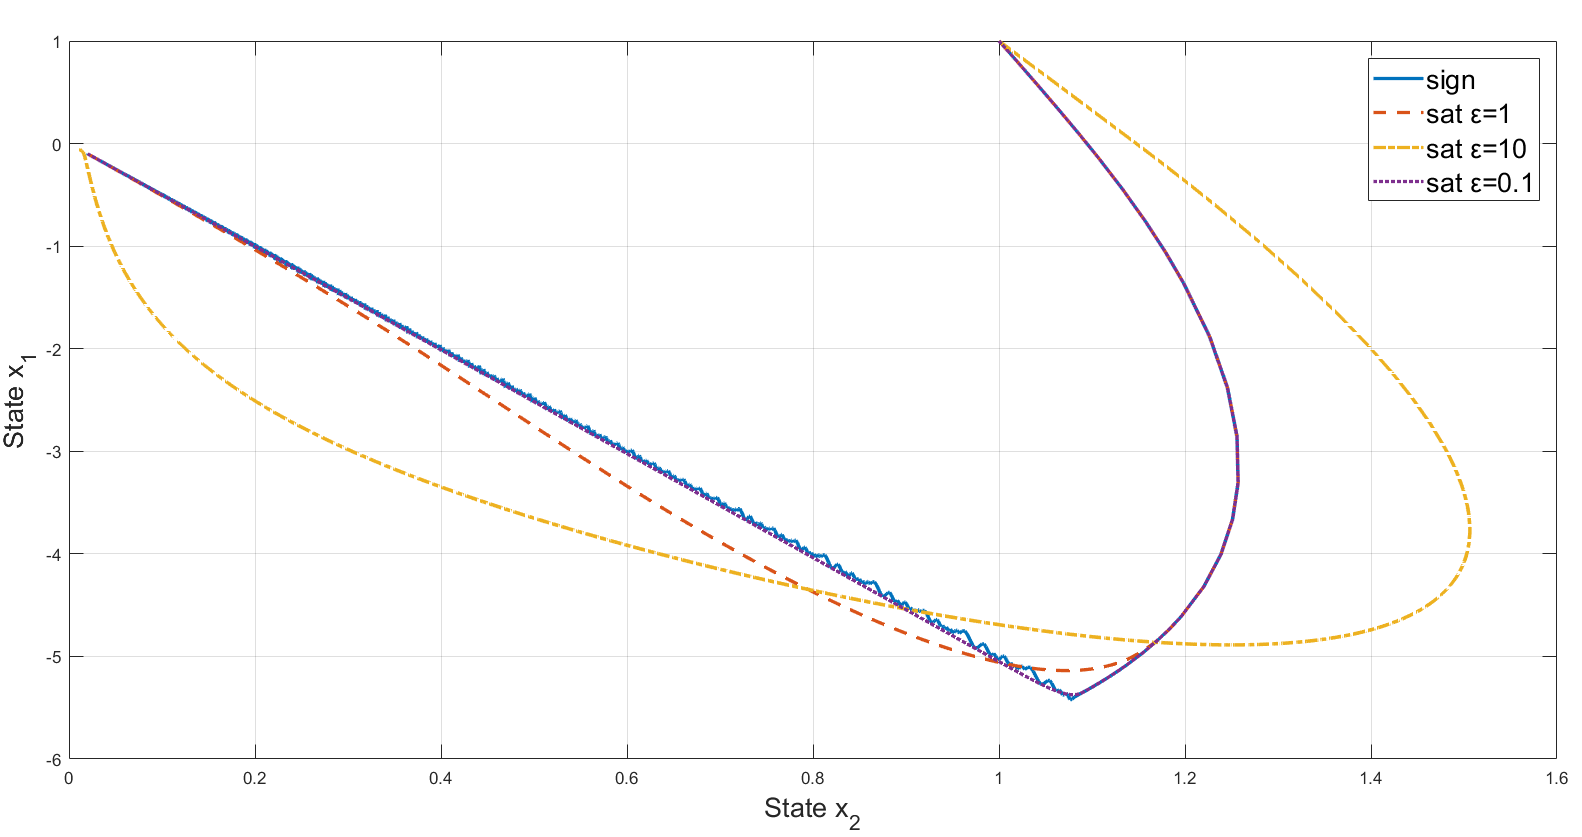
\includegraphics[scale=0.35]{figures/x1_x2_p4b.png}
	\centering
	\caption{State $x_1$ over $x_2$ of the closed-loop system using sliding mode control for various saturation values by altering $\epsilon$ and gain $K=0$.}
	\label{fig:x_1-x_2-smc}
\end{figure}
\end{solution}
\end{document}


